% LaTeX 2e Document.
% 
% $Id: sort.tex,v 1.6 2005/05/13 00:41:45 vdmtools Exp $
% 

%%%%%%%%%%%%%%%%%%%%%%%%%%%%%%%%%%%%%%%%
% PDF compatibility code. 
\makeatletter
\newif\ifpdflatex@
\ifx\pdftexversion\@undefined
\pdflatex@false
%\message{Not using pdf}
\else
\pdflatex@true
%\message{Using pdf}
\fi

\newcommand{\latexorpdf}[2]{
  \ifpdflatex@ #2
  \else #1
  \fi
}

\newcommand{\pformat}{a4paper}

\makeatother
%%%%%%%%%%%%%%%%%%%%%%%%%%%%%%%%%%%%%%%%

\latexorpdf{
\documentclass[\pformat,12pt]{article}
}{
\documentclass[\pformat,pdftex,12pt]{article}
}


\usepackage[dvips]{color}
\usepackage{longtable}
\usepackage{alltt}
\usepackage{graphics}
\usepackage{vpp}
\usepackage{makeidx}
\makeindex

\definecolor{covered}{rgb}{0,0,0}      %black
%\definecolor{not_covered}{gray}{0.5}   %gray for previewing
%\definecolor{not_covered}{gray}{0.6}   %gray for printing
\definecolor{not_covered}{rgb}{1,0,0}  %red

\newcommand{\InstVarDef}[1]{{\bf #1}}
\newcommand{\TypeDef}[1]{{\bf #1}}
\newcommand{\TypeOcc}[1]{{\it #1}}
\newcommand{\FuncDef}[1]{{\bf #1}}
\newcommand{\FuncOcc}[1]{#1}
\newcommand{\MethodDef}[1]{{\bf #1}}
\newcommand{\MethodOcc}[1]{#1}
\newcommand{\ClassDef}[1]{{\sf #1}}
\newcommand{\ClassOcc}[1]{#1}
\newcommand{\ModDef}[1]{{\sf #1}}
\newcommand{\ModOcc}[1]{#1}


\begin{document}
\vdmtoolsmanualscsk{VDM++ Sorting Algorithms}{2.0}

\section{Introduction}

This document contains a sorting example. The class diagram can be
seen in Figure \ref{inh}.  The structure of the example is known as
the \textit{strategy} pattern. This pattern defines a family of
algorithms, encapsulates each one and make them interchangeable. The
\textit{strategy} pattern lets the algorithm vary independently from
clients that use it. The \texttt{SortMachine} class is the client that uses the
different sorting algorithms. The \texttt{Sorter} class is an abstract class
that defines a common interface to all supported algorithms.


\begin{figure}[tbh]
\begin{center}
\mbox{}
\resizebox{12cm}{!}{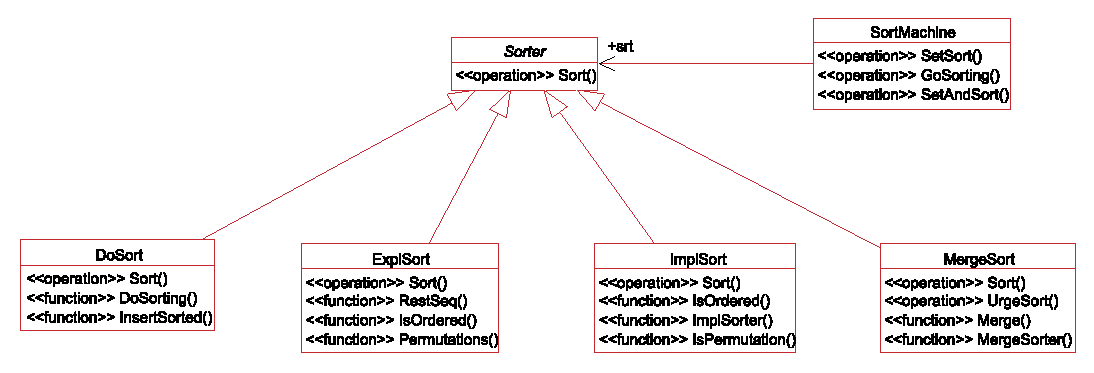
\includegraphics{inherit2}}
\caption{Class diagram for the sort example}\label{inh}
\end{center}
\end{figure}

\include{sortmachine.vpp}

\include{sorter.vpp}

\include{mergesort.vpp}

\include{dosort.vpp}

\include{implsort.vpp}

\include{explsort.vpp}

\newpage
\addcontentsline{toc}{section}{Index}
\printindex


\end{document}
